\documentclass[12pt,titlepage]{article}

\usepackage{mcgill,palatino,fancyhdr,listings}

\lhead{STAT201A -- Sec. 102}
\chead{HW \#4. }
\rhead{Steven Pollack -- 24112977}
\cfoot{\thepage}

\title{STAT201A -- Sec. 102 \\ Homework \#4. }
\author{Steven Pollack \\ 24112977}
\date{}

\usepackage{Sweave}
\begin{document}
\Sconcordance{concordance:stat201a_hw4.tex:stat201a_hw4.Rnw:%
1 13 1 1 0 106 1 1 58 1 23 1 18 1 20 1 21 27 1}

\maketitle

\pagestyle{empty}
\newpage
\pagestyle{fancy}

\paragraph{\#1.} Show that for fixed $n$, the binomial SD is largest when $p=1/2$. Please avoid calculus; the variance is an easily understood function of $p$. 
\begin{proof}
Recall that for a quadratic of the form $b-(x-a)^2$, a maximum is attained at $x=a$ (the point of the vertex). Thus, if we rewrite $p(1-p)$ as
\[
p(1-p) = p(1-p) - \frac{1}{4} + \frac{1}{4} = \frac{1}{4} -\left(p-\frac{1}{2}\right)^2
\]
 we see that our function is a concave down, quadratic with vertex at $p=1/2$. 

Tying this back to $SD(X)$, for $X \sim \text{Binomial}(n,p)$, we have that $SD(X) = \sqrt{npq}$, and thus $SD(X)^2 = \var(X) = np(1-p)$, which is maximized at $p=1/2$. And because $\sqrt{\cdot}$ is a monotonic function therefore optimizing $\sqrt{f(x)}$ is equivalent to optimizing $f(x)$, we see that $SD(X)$ is maximal at $p=1/2$. 
\end{proof}

\newcommand{\g}{\ord{P_{1}(A^{*})-P_{2}(A^{*})}}
\newcommand{\G}{\ord{P_{1}(A_{*})-P_{2}(A_{*})}}
\newcommand{\h}{\ord{P_{1}(B)-P_{2}(B)}}
\newcommand{\dist}{d(P_1,P_2)}
\renewcommand{\S}{\mathcal{S}}

\paragraph{\#2.} Let $\S$ be a finite set and let $P_1$ and $P_2$ be two probability distributions on $\S$. Let $\F$ be the set of all subsets of $\S$. Define the \textit{total variation distance} between $P_1$ and $P_2$ to be 
\[
\dist = \max\set{ A \in \F : \ord{P_1(A) - P_2(A)} }
\]
Thus, $d$ is the largest amount by which the two distributions differ, across all possible events. 

Show that, 
\[
\dist = \frac{1}{2}\sum_{x \in \S} \ord{P_1(x) - P_2(x)}
\]
There are many ways to do this. Here's on, but you are free to use any other.

Let $A^{*} = \set{ x \in \S : P_1(x) > P_2(x) }$, $A_{*} = \set{ x \in \S : P_1(x) < P_2(x) }$, and $A_{*}^{*} = \set{ x \in \S : P_1(x) = P_2(x)}$. The union of these disjoint sets is clearly $\S$. You should have a proof after you've investigated:
\begin{enumerate}
\item[(i)] the relation between $\g$ and $\sum_{x \in A^*} \ord{P_1(x) - P_2(x)}$
\item[(ii)] the relation between $\g$ and $\G$
\item[(iii)] whether the max in the definition of $\dist$ can be greater than $\g$. 
\end{enumerate}

\begin{proof} Defining the following sets:
\begin{align*}
A^{*} &= \set{ x \in \S : P_1(x) > P_2(x) } \\
A_{*} &= \set{ x \in \S : P_1(x) < P_2(x) } \\
A_{*}^{*} &= \set{ x \in \S : P_1(x) = P_2(x)}
\end{align*}
and it's clear that $\S = A^{*} \sqcup A_{*} \sqcup A_{*}^{*}$.  Furthermore, the finite size of $\S$ allows us to write 
\[
P_i(A^{*}) = P_{i}\left( \bigsqcup_{x \in A^{*}} \set{x} \right) = \sum_{x \in A^{*}} P_{i}(x) \qquad (i=1,2)
\]
Hence,
\begin{align*}
\ord{P_{1}(A^{*}) - P_{2}(A^{*})} &= \ord{ \sum_{x\in A^{*}} P_1(x) - \sum_{x \in A^{*}} P_{2}(x)} \\
&= \ord{ \sum_{x \in A^{*}} P_1(x) - P_2(x) } = \sum_{x \in A^{*}} \ord{P_1(x) - P_2(x)} = \sum_{x \in A^{*}} (P_1(x) - P_2(x))
\end{align*}
Similarly, 
\begin{align*}
\ord{P_1(A_{*}) - P_{2}(A_{*})} &= \ord{\sum_{x \in A_{*}} P_{1}(x) - P_{2}(x)} = \sum_{x \in A_{*}} \ord{P_{1}(x) - P_{2}(x)}
\end{align*}
Since $P_{1}(x) - P_{2}(x) = 0$ for all $x \in A_{*}^{*}$, we see that
\begin{align*}
\ord{P_1(A^{*}) - P_{2}(A^{*})}+\ord{P_1(A_{*}) - P_{2}(A_{*})} &= \sum_{x\in A^{*}}\ord{ P_1(x) - P_2(x)} + \sum_{x \in A_{*}} \ord{P_{1}(x) - P_{2}(x)} \\
&= \sum_{x \in \S} \ord{P_{1}(x) - P_{2}(x)}
\end{align*}

Now, suppose $\g > \G$:
\begin{align*}
\g > \G &\EQ P_1(A^*) - P_2(A^*) > P_{2}(A_*) - P_{1}(A_*) \\
&\EQ P_1(A^*) + P_{1}(A_*) > P_2(A^*) + P_2(A_*) \\
&\EQ 1 - P_1(A_{*}^{*}) > 1 - P_2(A_{*}^{*}) \\
&\EQ P_1(A_{*}^{*}) > P_2(A_{*}^{*})
\end{align*}
But, this is impossible, since $P_{1}(x) = P_{2}(x)$ for all $x \in A_{*}^{*}$. Thus, $\g \leq \G$. However, a symmetric argument shows that \[\G \leq \g\] and thus, 
\[
\g = \G
\]

Finally, we establish that $\dist = \g$; Let $B \in \F \setminus\set{A_{*},A^{*}}$ and suppose
\[
\h > \g = \G
\]
Then, 
\[
2 \h > \left(\g + \G\right) = \sum_{x\in\S}\ord{P_{1}(x) - P_{2}(x)}
\]
and hence\footnote{note: $\ord{P_1(B) - P_2(B)} = \ord{\sum_{x\in B}(P_1(x)-P_2(x))} \leq \sum_{x \in B}\ord{P_1(x) -P_2(x)}$}
\[
\h > \sum_{x \in \S\setminus B}\ord{P_{1}(x) - P_{2}(x)} \geq \ord{P_{1}(B^{c}) - P_{2}(B^{c})}
\]
However, 
\[
\ord{P_{1}(B^{c}) - P_{2}(B^{c})} = \ord{(1-P_{1}(B)) - (1-P_{2}(B))} = \ord{P_2(B) - P_1(B)}
\]
Thus, our assumption of strict inequality led us to the (nonsensical) conclusion that
\[
\h > \ord{P_2(B) - P_1(B)}
\]
so our max must be attained at $A^{*}$ and $A_{*}$. Thus, 
\[
\dist = \frac{1}{2} \times 2\dist = \frac{1}{2}\left(\g + \G \right) = \frac{1}{2} \sum_{x\in\S}\ord{P_{1}(x) - P_{2}(x)}
\]
\end{proof}







\paragraph{\#3.}
\begin{figure}[thbp!]
\centering
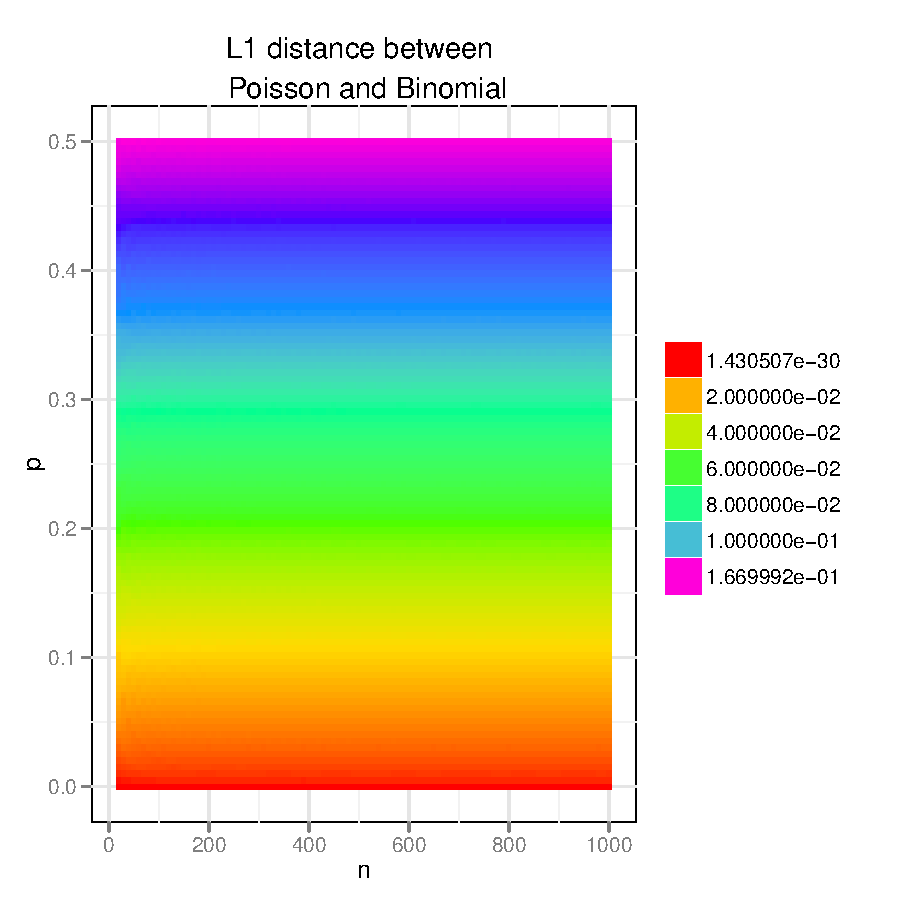
\includegraphics[width=0.6\textwidth, trim = 5mm 0mm 10mm 6mm, clip]{stat201a_hw4-plot_L1_poisson.pdf} \\
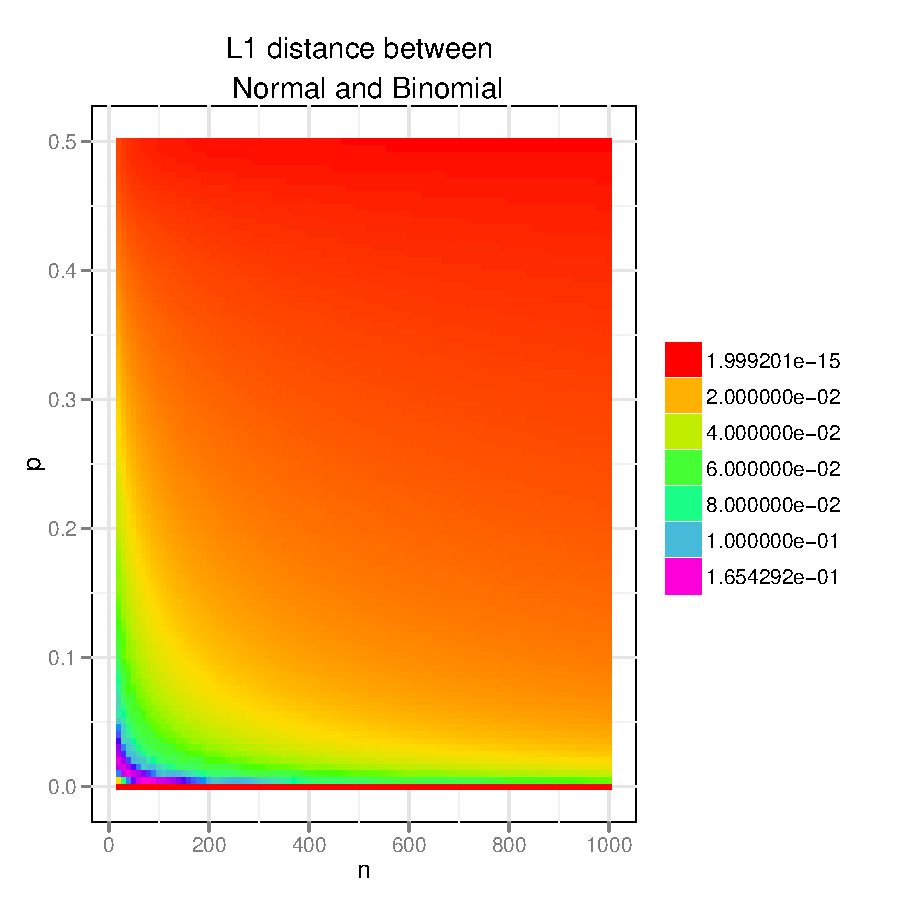
\includegraphics[width=0.6\textwidth,trim = 5mm 0mm 10mm 6mm, clip]{stat201a_hw4-plot_L1_normal.pdf} 
\caption{A graphical comparison of the $L_1$ distance between the two distributions as a function of $(n,p)$. Note: red is lower in magnitude than violet.}
\end{figure}

\begin{figure}[thbp!]
\centering 
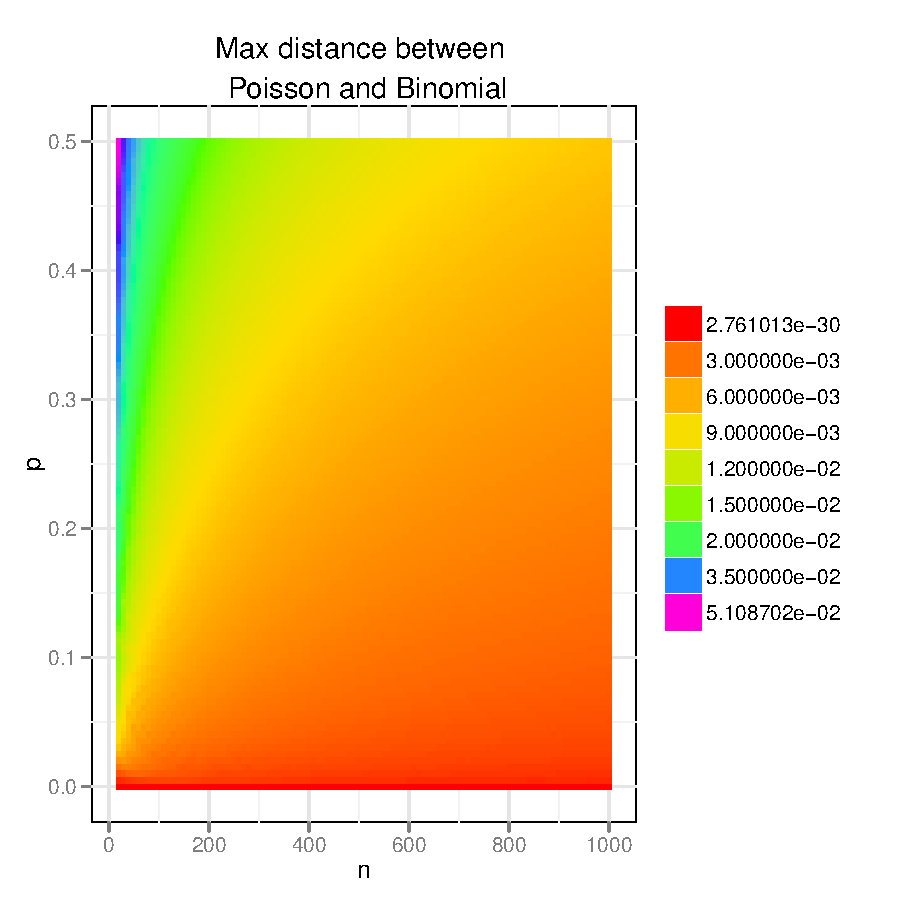
\includegraphics[width=0.6\textwidth, trim = 3mm 0mm 10mm 6mm, clip]{stat201a_hw4-plot_sup_norm_poisson.pdf} \\
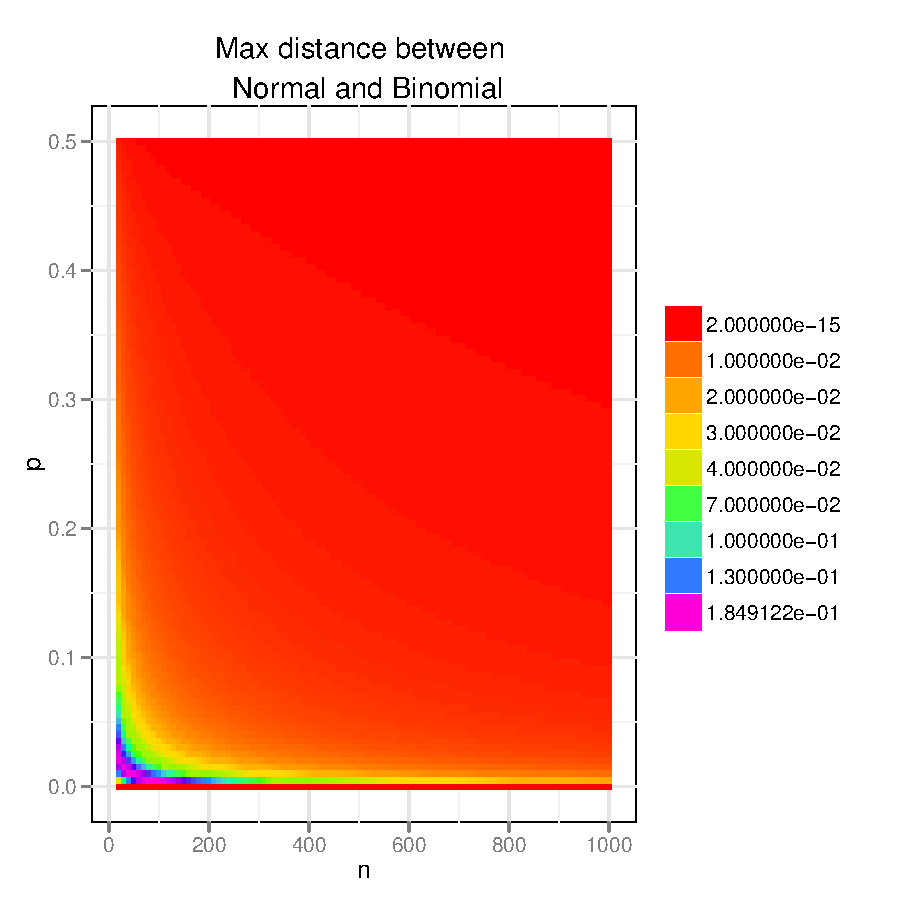
\includegraphics[width=0.6\textwidth, trim = 3mm 0mm 10mm 6mm, clip]{stat201a_hw4-plot_sup_norm_normal.pdf}
\caption{A graphical comparison of the $L_{\infty}$ distance between the two distributions as a function of $(n,p)$.}
\end{figure}

So, a first look at the $L_1$ distance comparisons in figure 1, immediately indicates that there is a convex region in the (half) ($n$,$p$)-plane where the normal approximation is far-superior to the Poisson. Doing some rough linear regression, we can use the function $p = 0.126\exp(-2.32\times10^{-3}n)$ (for $n \geq 20$) as one boundary curve of this region. 

Furthermore, the graphics in figure 2 indicate that this convex region is good, not only for gaging when the normal approximation is $L_1$-superior, but for when it is $L_{\infty}$ superior. Hence, I feel comfortable employing the following ``rule of thumb'': if $(n,p) \in [20,10^{3}]\times[0,1]$, and $p \leq 0.126\exp\set{-2.32\times10^{-3} n}$, then go with the Poisson approximation. Otherwise, use the normal.

Note: $e^{-.00232} \approx 0.998$ and $0.126 \approx 1/8$, so we can roughly peg our rule of thumb to something like
\[
8 p \leq 0.998^{n} %= (1-.002)^{n} = \SUM{j}{1}{n}\binom{n}{j}(-.002)^{j} = (-1)^{j}10^{-3j} 2^j
\]
\newpage
\newpage 
\section*{R Code}
\lstinputlisting[language=R,breaklines=True]{../stat201a_hw4.R}
\end{document}
